\documentclass{beamer}[10]


%
% macro
%

\usepackage{pgf}
\usepackage[english]{babel}
\usepackage[utf8]{inputenc} % use unicode chars
\usepackage{lmodern}% http://ctan.org/pkg/lm
\usepackage{beamerthemesplit}
\usepackage{graphics,epsfig,subfigure}
\usepackage{url}
\usepackage{srcltx}
\usepackage{hyperref}
\usepackage[mathescape,escapeinside=||]{minted}
\usepackage{import}
\usepackage{mathtools}
\usepackage{amsmath}
\usepackage{color}
%\usepackage[beamer]{hf-tikz}
\usepackage{xfrac}
\usepackage{makeidx}
\usepackage{multicol}

%\showboxdepth=5
%\showboxbreadth=5

% Slides in 16:9
\usepackage[orientation=landscape,size=custom,width=16,height=9,scale=0.5,debug]{beamerposter} 

%
% Macros
%
\definecolor{darkred}{rgb}{0.55, 0.0, 0.0}
\definecolor{light-gray}{gray}{.80}
\definecolor{light-yellow}{rgb}{255,255,153}
\definecolor{alizarin}{rgb}{0.82, 0.1, 0.26}
% colorized font
\newcommand{\red}[1] {{\color{red} #1}}
\newcommand{\darkred}[1] {{\color{darkred} #1}}
\newcommand{\blue}[1] {{\color{blue} #1}}
\newcommand{\green}[1] {{\color{green} #1}}
\newcommand{\gray}[1] {{\color{gray} #1}}
\newcommand{\grey}[1] {{\color{gray} #1}}

\newcommand{\hearts} {\red{$\heartsuit$}}
\newcommand{\diamonds} {\red{$\diamondsuit$}}
\newcommand{\spades} {$\spadesuit$}
\newcommand{\clubs} {$\clubsuit$}
\newcommand{\pyoptional}[1]{\diamonds #1 \diamonds}

\newcommand{\deltasum}[1]{\sum (#1 - \bar{#1})}
\newcommand{\deltasumsq}[1]{\sum (#1 - \bar{#1})^{2}}

%
% Take care of the newline after \frametitle
%
\newenvironment{pyframe}[1]
{\begin{frame}[fragile,environment=pyframe]\frametitle{#1}
 
}
{\end{frame}}


% environments
\newminted{py}{mathescape,escapeinside=||}% 
\newminted{bash}{mathescape,escapeinside=||}%

% python highlights: module, method
\newcommand{\pymodule}[1]{\darkred{\textbf{#1}}}
\newcommand{\pyfunction}[1]{\textit{#1}}
\newcommand{\keyword}[1]{\texttt{#1}}
\newcommand{\pyver}[1]{\colorbox{yellow}{#1}}
\newcommand{\typeonly}[1]{\colorbox{green}{#1}}
\newcommand{\pyvers}[1]{\raisebox{0em}{\colorbox{yellow}{#1}}}
\newcommand{\code}[1] { \texttt{#1} }

% special symbils
\newcommand{\mymapsto}{\operatornamewithlimits{\longmapsto}}

\makeatletter
\newcommand{\xMapsto}[2][]{\ext@arrow 0599{\Mapstofill@}{#1}{#2}}
\def\Mapstofill@{\arrowfill@{\Mapstochar\Relbar}\Relbar\Rightarrow}
\makeatother




%
% style
%

\setbeamercovered{transparent}
\mode<presentation>

%\geometry{top=5pt, margin=5pt}
%The outertheme defines the head and the footline of each slide
% \setbeamercolor{block title}{bg=orange}
% \useinnertheme{circles}
% \useoutertheme{split}
%\beamertemplatenavigationsymbolsempty

%\usetheme[numbers,totalnumber,compress,sidebarshades]{Babel}
\setbeamertemplate{headline}{
 \leavevmode%
  \hbox{%
%,bb=0 0 5cm 2cm
    \hspace{5pt}\includegraphics[height=1.2cm]{logo.eps}
    \hspace{240pt}\includegraphics[height=1.2cm]{logo.eps}
    }
}
\setbeamertemplate{footline}{
\noindent\textbf{\hspace{5pt}\insertsection \insertsubsection\hfill}\textbf{\hfill{\color{gray}\insertshortauthor}\hfill}\textbf{\hfill }
   % \textline[t]{ \insertsection  \insertsubsection}{\gray{\insertshortauthor}}{right}
}
%\useinnertheme[shadow=false]{rounded}
% frametitle
\setbeamertemplate{frametitle}[default][center]
\setbeamercolor*{frametitle}{bg=white,fg=gray,parent=palette primary}
\setbeamerfont{frametitle}{series=\bfseries,size={\fontsize{16}{8}}}
% table of contents
\setbeamercolor{section in toc}{fg=black} % series=\bfseries,size={\fontsize{16}{8}}}
%\setbeamercolor{section/subsection in toc}{fg=black}
%\setbeamercolor{subsection in toc}{fg=black}
%\setbeamerfont{section in toc}{fg=black} % series=\bfseries,size={\fontsize{16}{8}}}
%\setbeamerfont{section/subsection in toc}{fg=black}
%\setbeamerfont{subsection in toc}{fg=black}

%title
\setbeamercolor{title}{fg=black,bg=white}
\setbeamerfont{title}{series=\bfseries,size={\fontsize{24.88}{32}}}
%subtitle
\setbeamercolor{subtitle}{fg=gray}
\setbeamerfont{subtitle}{series=\bfseries,size={\fontsize{14}{}}}
%titlepage
\setbeamertemplate{title page}[default][center]
% bullets
\setbeamercolor{itemize item}{fg=gray}
\setbeamertemplate{itemize items}[circle]
\setbeamercolor{itemize item}{fg=light-gray}
\setbeamercolor{itemize items}{fg=light-gray}
% enumerations
\setbeamercolor{enumerate item}{fg=black}
\setbeamercolor{local structure}{fg=black}

%
% increase itemize spacing
%
%\newlength{\wideitemsep}
%\setlength{\wideitemsep}{\itemsep}
%\addtolength{\wideitemsep}{14pt}
%\let\olditem\item
%\renewcommand{\item}{\setlength{\itemsep}{\wideitemsep}\olditem}

  % \usecolortheme[named=orange]{structure}
  % \useinnertheme{circles}
  % \usefonttheme[onlymath]{serif}
\setbeamercovered{transparent}
  % \setbeamertemplate{blocks}[rounded][shadow=true]

\makeindex


% Apply DRAFT watermark
\usepackage{draftwatermark}
\setbeamercolor{background canvas}{bg=}%transparent canvas

\title{Orchestrating MySQL with Python and Docker}
\subtitle{C4P EuroPython 2015, $22^{th}$ July - Bilbao}
\author{Roberto Polli - \href{mailto:roberto.polli@par-tec.it}{roberto.polli@par-tec.it}}
\date{21-27 July 2015}
\institute{Par-Tec Spa - Rome Operation Unit\\
    P.zza S. Benedetto da Norcia, 33\\
    00040, Pomezia (RM) - www.par-tec.it}

%
%
\begin{document}

%% cover
\frame{\titlepage 
\vspace{-0.5cm}
}


%% agenda
\frame{\frametitle{Agenda}
\begin{multicols}{2}
\tableofcontents
\end{multicols}
}


%% Starting doc
\section{Intro}
\frame{ \frametitle{Who? What? Why?}
\begin{itemize}

\item Manage, replicate, scale and provision databases with mysql-fabric.
\\
\\
\item Roberto Polli - Solutions Architect @ par-tec.it. Loves writing in C,
Java and Python. Red Hat Certified Engineer and Virtualization
Administrator.
\\
\\
\item Par-Tec – Proud sponsor of this talk ;) Contributes to various FLOSS. \\
Provides expertise in IT Infrastructure \& Services and \\ Business Intelligence
solutions + Vertical Applications for the financial market.

\end{itemize}
}

\begin{pyframe}{EuroPython 2015 C4P}
Training is work in progress. Slides are just teaser and will be completed if the training will be accepted.
\\
I am open to suggestions an improvements!
\\
Support this training and have your say ;)
\href{http://github.com/ioggstream/python-course/scaling-mysql-with-python}{github.com/ioggstream/python-course/scaling-mysql-with-python}
\end{pyframe}

%
%
%
\begin{pyframe}{Setup}
Install Docker
\begin{bashcode}
sudo apt-get install lxc-docker || \
yum -y install docker
\end{bashcode}
Download the course scripts
\begin{bashcode}
git clone https://github.com/ioggstream/mysql-community
cd mysql-community/fabric
\end{bashcode}
Install requirements and setup environment
\begin{bashcode}
pip install -r requirements.txt
docker-compose up
# this will download docker images!
\end{bashcode}
\end{pyframe}


%
% Docker 101
%
\section{Introducing Docker \& Compose: 30'}
\begin{pyframe}{Docker}
A brief docker tutorial based
on the busybox image.
Setting images, hostnames and environment variables.

\begin{bashcode}
$ docker run [--rm] -ti --name=test busybox /bin/bash
$ docker exec -ti  test /bin/bash
...
\end{bashcode}

OT: nat, entrypoint, ...
\end{pyframe}


\begin{pyframe}{Docker Compose}
A brief docker-compose tutorial:
describing containers via yml

\begin{columns}[t]
\column[t]{.5\linewidth}
Running the provided services
using docker-compose.
\\
Clean up all containers with
\begin{bashcode}
docker-compose kill
# and
docker-compose rm -vf
\end{bashcode}
\column[t]{.5\linewidth}
\begin{pycode}
#  docker-compose start db
db:
 image: ioggstream/mysql-community
 volumes:
   - ./:/code
 environment:
   - MYSQL_ROOT_PASSWORD=root
 command: [
   'mysqld',
   '--defaults-file=/code/my.cnf'
 ]
\end{pycode}
\end{columns}

\end{pyframe}


\begin{pyframe}{Docker Compose}
Scaling services with compose.
\begin{columns}[t]
\column{.4\linewidth}
\begin{bashcode}
$ docker-compose scale db=1
Creating fabric_slave_1..
Starting fabric_slave_1...

$ docker-compose scale db=8
Creating fabric_slave_2..
..
Starting fabric_slave_8...

$ docker-compose scale db=4
...
\end{bashcode}
\column{.4\linewidth}
\begin{bashcode}
$ docker-compose ps
     Name          Command     State
-------------------------------------
fabric_fabric_1   /run.sh...   Up
fabric_db_1       /run.sh...   Up
..
fabric_db_4       /run.sh...   Exit 0

$ docker inspect -f ...
/fabric_db_3 172.17.0.4
/fabric_db_2 172.17.0.3
/fabric_db_1 172.17.0.2
/fabric_fabric_1 172.17.0.5

\end{bashcode}
\end{columns}

\end{pyframe}


%
% MySQL
%
\section{MySQL Replication: 20'}
\begin{pyframe}{MySQL Replication 101}
Advantage of replication:
\begin{itemize}
  \item scaling reads
  \item high availability
  \item simplify backups
\end{itemize}
\end{pyframe}


\begin{pyframe}{MySQL Replication 101}
Overview of MySQL Replication:
\begin{itemize}
\item master creates a changelog (binlog),
% by default binlog never expires
\item slaves download and apply it.
\item every transaction has a global id (GTID).
\item Asynchronous and Semi-Synchronous replication.
\end{itemize}
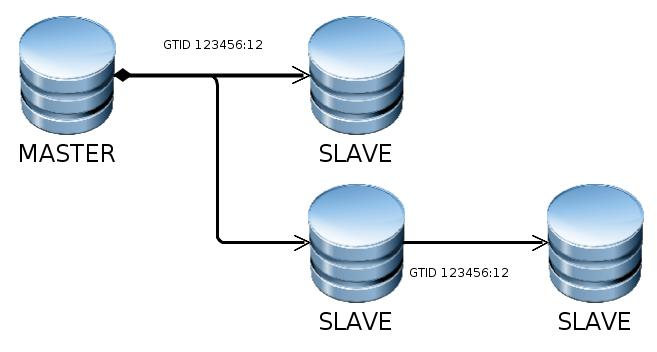
\includegraphics[height=4cm]{images/mysql-propagate-gtid.jpg}
\end{pyframe}


\iffalse
\begin{pyframe}{Replication 2.0}
MySQL 5.6+ replication is based on Global Transaction ID
\begin{itemize}
\item Every server has a unique UUID \\
\code{3E11FA47-71CA-11E1-9E33-C80AA9429562}

\item This makes every TransactionID a Global one
\code{3E11FA47-71CA-11E1-9E33-C80AA9429562:32}
\end{itemize}
GTIDs simplify replication and synchronization (one or more slide)
\end{pyframe}


\begin{pyframe}{Configuring replication}
\begin{itemize}
\item Replication agreement is configured on the slave only;
\item The slave connects to the master with a provisioned
 user and gets its changelog (binlog);
\item Incomplete binlogs require a slave initialization.
\end{itemize}
\end{pyframe}
\fi


\begin{pyframe}{MySQL Replication 101}
Running mysql with the provided and commented
configuration file \href{http://github.com/ioggstream/mysql-community/fabric}{my.cnf}
\\
Consistency parameters (more to come).
\\
Replication parameters (crash-safe replication).
\\
Replication start/stop/status.
%Create a master-slave replication agreement.
%\code{SLAVE START; SLAVE STOP; SHOW SLAVE STATUS \G; SHOW MASTER STATUS;}
\end{pyframe}


%
% Fabric
%
\section{MySQL Fabric: 10'}
\begin{pyframe}{Fabric - HLA}
Fabric is a python framework for managing, replicating, sharding and scaling mysql servers.
\begin{itemize}
\item aggregate servers in high availability groups
\item configure single-master replication topologies
\item monitor and heal failures
\item director for rw/split and sharding
\item fabric connectors (caching db topology)
\end{itemize}
\end{pyframe}
%http://mysqlmusings.blogspot.it/2013/10/mysql-fabric-high-availability-groups.html


\begin{pyframe}{Fabric - HLA}
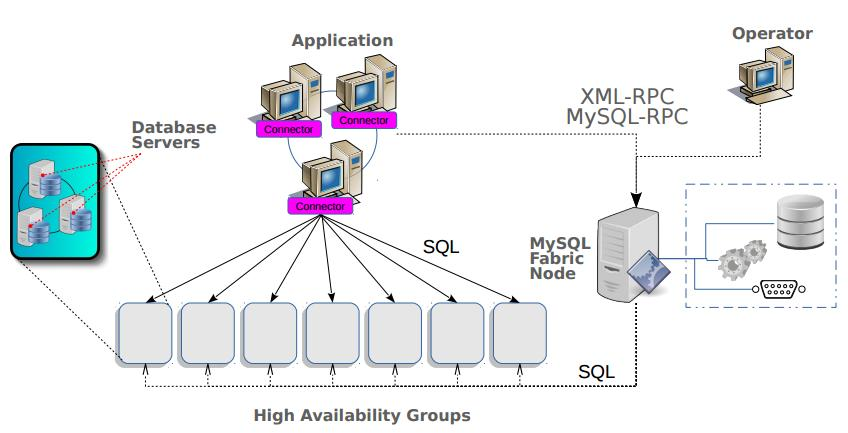
\includegraphics[height=6.6cm,width=12cm]{images/mysql-fabric-hla.jpg}
\end{pyframe}


\subsection{Fabric installation \& setup: 20'}
\begin{pyframe}{Fabric \& Python Utilities - get it}
Download and browse the latest sources
\begin{columns}[t]
\column[t]{.5\linewidth}
    %|\href{https://dev.mysql.com/get/Downloads/MySQLGUITools/mysql-utilities-1.6.1.tar.gz}{
    \begin{bashcode}
    # Already provided in the
    #  docker image!
    wget http://bit.ly/1CxNuZe
    tar xf mysql-utilities-1.6.1.tar.gz
    python setup.py install
    \end{bashcode}
\column[t]{.5\linewidth}
\begin{bashcode}
   |-- mysql
   |-- connector
   |   |-- django
   |   `-- fabric
   |-- fabric
   |   |-- protocols
   |   |-- providers
   |   `-- services
   `-- utilities
\end{bashcode}
\end{columns}

\end{pyframe}

\iffalse
Fedora / CentOS / RHEL 7
    \begin{bashcode}
    yum -y install \href{https://dev.mysql.com/get/mysql-community-release-el7-5.noarch.rpm}{http://bit.ly/1yhSViu} # MySQL Community repo
    yum -y install mysql-utilites
    \end{bashcode}
\fi



\begin{pyframe}{Setup the lab}
Setup and check the course environment.
\begin{bashcode}
$ docker-compose up -d
$ docker-compose ps
$ docker inspect -f '{{.Name}} {{.NetworkSettings.IPAddress}}'
\end{bashcode}

Check the 'fabric' container: we will access all servers from this
 one which includes *all* mysql tools and utilities.
\begin{bashcode}
$ docker exec -ti fabric_fabric_1 /bin/bash
fabric$
\end{bashcode}
\end{pyframe}


\begin{pyframe}{Setup - II}
Image with the training infrastructure (fabric, database and docker nodes).
\\
Configure credential in $encrypted$ (mysql\_config\_editor)
 or clear-text (my.cnf) files to avoid wasting time during
the training.
 \\
\end{pyframe}

%\begin{pyframe}{Setup - III}
%*empty*
%\end{pyframe}

\begin{pyframe}{Introducing mysqlfabric}
The training covers:
\begin{itemize}
\item \code{manage [setup|start|ping|stop|teardown]}
\item group - manage high availability groups
\item server - manage, clone, provision and decommission servers
\item provider - manage server providers (eg. openstack, ...)
\end{itemize}
Further functionalities:
\begin{itemize}
\item statistics, dump, role, user,
\item threat, sharding, snapshot, event
\end{itemize}
\end{pyframe}


\begin{pyframe}{Test Driven Installation}
The installation is test-driven via a provided nose script.
Students will be guided in fixing all the tests.
Testing fabric installation (node reachability, user existence, ...)

\begin{bashcode}
fabric$ cd /code
fabric$ nosetests -v
test_root_access_nodes('m.docker', {'password': 'root', 'user': 'root'}) ... fail
..
test_fabric_access_nodes('m.docker', {'password': 'fabric', 'user': 'fabric'}) ... fail
...
test_fabric ... ERROR
test_fabric_node ... ERROR
\end{bashcode}
\end{pyframe}



\begin{pyframe}{Test Driven Installation}
Setup fabric server via fabric.cfg . \\
Students will be guided in fixing all the tests.

\begin{bashcode}
$ mysqlfabric manage setup / start
$ mysqlfabric ping ...
\end{bashcode}
\end{pyframe}


\section{Replication Groups: 30'}
\begin{pyframe}{Create a Group}
Create a replication group and adding
servers. \\

Promoting one server as a master. \\
\code{mysqlfabric dump servers}
\\
Adding spare servers. \\

Monitoring failover. \\
\begin{bashcode}
# mysqlfabric group [create|promote|activate] $GROUP
...
\end{bashcode}
\end{pyframe}


\begin{pyframe}{}
Import data and check replication status using python tools.

\begin{bashcode}
mysqldbimport --server=$MASTER ... sakila.sql
mysqldbcompare --server1=$MASTER --server2=$SLAVE \
  --all
\end{bashcode}
\end{pyframe}


\begin{pyframe}{Connecting to a group}
Configure python clients
\begin{pycode}
from mysql.connector import connect, fabric
c = connect(fabric={host: .., port: .., user: ..},
    autocommit=True,
    database='sample', **sql_user)
c.set_property(mode=fabric.MODE_READWRITE, group="my-cluster-1")
\end{pycode}
\\
Test R/W split and balancing with nose.
\begin{bashcode}
nosetests -vs test_script.py -m rwsplit
\end{bashcode}
\end{pyframe}


\section{Troubleshooting: 20'}
\begin{pyframe}{Provisioning a new slave}
When binlogs have been purged / expired, you need to
import from another server.\\

Caveats on big databases. \\

Provision a new slave with
\begin{bashcode}
mysqlfabric server clone $GROUP $TARGET
\end{bashcode}

Provision a new slave with python utilities
\begin{bashcode}
# Remove all replica configurations
#  on the slave..
mysql -h$SLAVE -e 'STOP SLAVE;RESET MASTER;'

# ..and reinitialize it
mysqldbcopy --source=$MASTER --destination=$SLAVE
    --rpl-user=fabric:fabric --rpl=master
    --all --drop-first
\end{bashcode}
\end{pyframe}


\iffalse
    \begin{pyframe}{Provisioning a new slave}
    Provision a new slave in two steps (eg. large database or requiring tweaks)
    \begin{itemize}
    \item check that replica user is provisioned on the master;
    \item create a custom dump.sql;
    \item add --rpl=master;
    \end{itemize}
    \begin{minted}
    cat > data.sql <<EOF
    -- ignore previous changelogs
    -- and trust the backup only
    STOP SLAVE;
    RESET MASTER;

    EOF

    mysqldbexport >> data.sql \
     --server=root:pass@master \
     --rpl-user=repl:rpass \
     --export=master \
     --rpl=master \
     --all

    mysqldbimport --server=root:root@slave \
     data.sql
    \end{minted}
    \end{pyframe}
\fi


\section{Failover: 20'}
\begin{pyframe}{Enabling and Testing Failover}
Enabling failover and stopping a master. \\

Checking automatic failover. \\
\begin{bashcode}
#nosetests -vs --nologcapture fabric-poc.py -m failover &
#mysqladmin shutdown -h $MASTER
\end{bashcode}

Re-ingesting a failed master. \\
\begin{bashcode}
mysqlfabric server set_status  f484d0ed-ecea-11e4-9118-0242ac110039  spare
mysqlfabric server set_status  f484d0ed-ecea-11e4-9118-0242ac110039  secondary
\end{bashcode}
\end{pyframe}


\section{Provisioning: 20'}
\begin{pyframe}{Provisioning new container via docker}
Show the provisioning interface (docker, openstack). \\

\begin{pycode}
# mysql.fabric.providers.dockerprovider
class MachineManager(AbstractMachineManager):
    """Manage Docker Containers."""
    def create(self, parameters, wait_spawning):
        ...
    def search(self, generic_filters, meta_filters):
        ...
    def destroy(self, machine_uuid):
        ...
\end{pycode}
\end{pyframe}


\begin{pyframe}{Docker Provisioning}

Provisining and deleting containers. \\

Adding provisioned container to ha groups. \\

\begin{bashcode}
# Register a provider (requires docker in http)
mysqlfabric provider register mydocker \
    user password \
    http://172.17.42.1:2375  \
    --provider_type=DOCKER

# Create new server
mysqlfabric server create mydocker \
    --image=name=mysql-fabric   \
    --flavor=name=v1            \
    --meta=command="mysqld --log-bin=foo"

# List servers
mysqlfabric server list docker
\end{bashcode}
\end{pyframe}


\begin{pyframe}{Docker Provisioning}
Improving the docker provisioning.

Curious? Vote this training!

\begin{bashcode}
...
\end{bashcode}
\end{pyframe}

\iffalse
\begin{pyframe}{Title}
\begin{bashcode}
#
\end{bashcode}
\end{pyframe}
\fi




\begin{pyframe}{Wrap Up}
\begin{itemize}
\item Replication is easier with Fabric and MySQL 5.6
\item You can clone servers
\item Failover is just one command ahead
\item You can't re\-ingest failed masters (luckily;)
\item Try Fabric with Docker!
\end{itemize}
\end{pyframe}


\begin{pyframe}{That's all folks!}
\begin{center}
Thank you for the attention! \\\\
\insertauthor
\end{center}
\end{pyframe}


\end{document}
